
%TROND:

The prefetcher is an attempt to investigate an alternative to the Delta-Correlating Prediction Tables (DCPT) approach by Granaes, Jahre and Natvig \cite{reference:jahre}. The original DCPT algorithm is described in the "Related Works" section. A weakness of this approach is (arguably) that it bases the prefetch address on the first similar delta pattern it finds. This makes the prefetcher somewhat vulnerable to alternating patterns and irregularities in general. If the access pattern makes a sudden leap in an otherwise regular pattern, not only will the prefetcher miss the irregular access, it is guaranteed to miss the next access after that when the pattern goes back to normal. This example is illustrated in Table \ref{table:breakDCPT}. Access number 6 breaks the pattern, and misses. Because the next fetch is based on access 6's delta, this also misses. This problem could be solved by a more democratic approach, where the most common "next delta" is used instead of the previous. 
Another different approach that was of interest to explore was to base the delta values on the addresses of the cache misses alone, instead of linking these to the address of the responsible instruction. This was an experiment to see whether the memory saved by omitting the extra program counter (PC) address would pay off due to the possibility of storing a larger number of deltas.
\begin{table}[!t]
\renewcommand{\arraystretch}{1.3}
\caption{}
\label{table:breakDCPT}
\centering
\begin{tabular}{|r|r|r|r|l|}
\hline
\bfseries Access & \bfseries Address & \bfseries Delta & \bfseries Fetch~Issued & \bfseries Previous~Result\\
\hline
\hline
%Access & Address & Delta & Fetch issued & Previous result\\
1 & ... & ... & ... & ...\\
2 & 1000 & 10 & 1010 & Hit\\
3 & 1010 & 10 & 1020 & Hit\\
4 & 1020 & 10 & 1030 & Hit\\
5 & 1030 & 10 & 1040 & Hit\\
6 & 1050 & 20 & 1070 & Miss\\
7 & 1060 & 10 & - 	 & Miss\\
8 & 1070 & 10 & 1080 & -\\
9 & 1080 & 10 & 1090 & Hit\\
\hline
\end{tabular}
\end{table}

This democratic and alternative approach is what the prefetcher described in this report implements. To achieve this, the structure of the reference table needs a major change. Instead of the linear array with an offset used in DCPT, this prefetcher utilizes a dynamic 2d array, resembling a sparse matrix. The algorithm is fired every time the program tries to access the cache. The access is logged, and the leap from the previous memory access address (the delta value) is stored in the database. The prefetcher then performs a lookup for the current address, and as the original DCPT, it determines the next delta from the two previous. If an entry is found for this delta combination, a prefetch is issued. If on the other hand no combination is found, the algorithm stores the cache miss address, and proceeds without issuing a prefetch. An alternative to this would have been to use sequencial fetching when these situations occur, but to minimize the risk of unnecessary memory operations this was not implemented. This decision will directly impact the number of overall fetches resulting in a smaller total, which will affect the performance statistics of the algorithm. This is further explained in the discussion section.   

The preferred delta leap on fetch N is determined by delta(N - 1) and delta(N - 2), the length of the two leaps before this one. Delta(N - 2) is put on the Y-axis of the sparse matrix, while delta(N - 1) is mapped along the X-axis. A binary search algorithm searches along the Y-axis (implemented as a C++-std::deqeue) for the delta(N - 2) entry. This entry is implemented as a C++-class containing the delta value and a new std::deque, which contains elements representing all the delta(N-1) entries ever to appear after the given delta(N - 2). The binary search algorithm is then applied to this inner deque, and returns an X-axis element. This element contains the delta(N - 1) value, the proposed next delta and a score for this combination. The "next delta" found in this X-axis element determines the address of the fetch. What makes this algorithm more "democratic" is the scoring of delta values. When a "next delta" is proposed for a delta combination, this proposition gets a start score. The next time the combination appears, the proposed next delta is applied. If the prefetch is a hit, the score increases, if it's a miss, it decreases. When a score gets below a given threshold, the proposition is replaced by the most recent candidate. 

\begin{figure}[h!]
	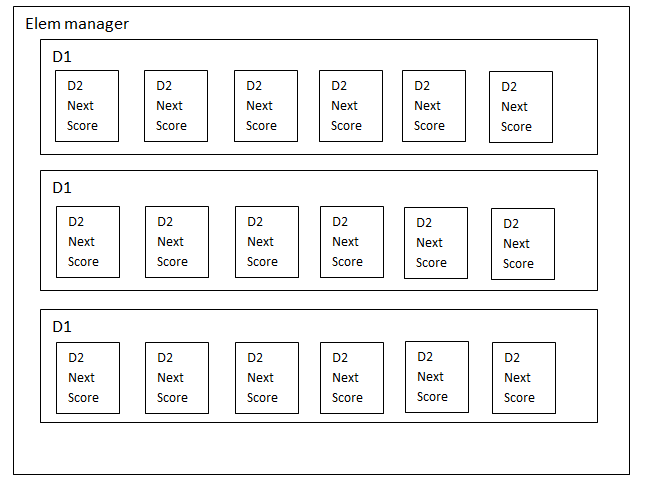
\includegraphics[width=3.5in]{table3}
	\caption{Overview over combination-pool datastructure}
	\label{graph:combpool}
\end{figure}



To accommodate to an 8kB memory cap, an upper element count threshold is applied. When the count exceeds this limit, the combination with the lowest score is removed from the structure, and replaced by a new element. This only applies if the lowest score is below a given kick threshold. This is to avoid altering a strong set of elements. In addition to the hit/miss scoring, all elements get deducted one point per memory access, meaning that old, unused combinations are more likely to be abandoned than fresh entries.

The entire algorithm is described in pseudo code in Algorithm \ref{alg:lol}. \\\\
\begin{algorithm}
\caption{The prefetch\_access(addr) implementation}
\label{alg:lol}
\begin{algorithmic}
\STATE static $delta[]$
\STATE static $total\_fetches \gets 0$
\STATE $delta \gets addr - prev\_addr$
\STATE
\STATE $//apply$ $previous$ $result:$
\STATE Elem $elem \gets$ find\_elem($delta[prev]$, $delta[prev - 1]$)
\IF{$elem$ == $NULL$} 
\STATE{$elem \gets$ add\_combination($delta[prev]$, $delta[prev - 1]$)}
\ENDIF
\IF{$delta$ == $elem$.$delta$}
\IF{$elem$.$score$ \textless $ total\_fetches$ + $BASE\_SCORE$}
\STATE{$elem$.$score += total\_fetches$ + $BASE\_SCORE$}
\ELSE
\STATE{$elem$.$score += HIT\_SCORE\_BOOST$}
\ENDIF
\ELSE
\STATE{$//check$ $whether$ $to$ $change$ $elem$.$delta$}
\IF{$elem$.$score$ \textless $ (SCORE\_KICK\_THRSLD$ + $total\_fetches)$}
\STATE{$elem$.$delta \gets$ $delta$}
\STATE{$elem$.$score \gets$ $BASE\_SCORE$ + $total\_fetches$}
\ELSE
\STATE{$elem$.$score -=$ $MISS\_SCORE\_PUNISHMENT$}
\ENDIF
\ENDIF
\STATE
\STATE $//find$ $next$ $delta:$
\STATE Addr $next\_fetch \gets$ get\_delta($delta[prev]$, $delta$)
\IF{is\_valid($next\_fetch$) \AND \NOT in\_cache($next\_fetch$)}
\STATE issue\_prefetch($next\_fetch$)
\ENDIF
\STATE
\STATE $//prep$ $for$ $next$ $run$
\STATE $delta[last - 1] \gets delta[last]$
\STATE $delta[last] \gets delta$
\STATE $total\_fetches++$
\end{algorithmic}
\end{algorithm}


